\documentclass[12pt]{report}
\title{Outils Data : Comment améliorer leur accessibilité pour les populariser ?}
\author{Enzo Bonnal}
\date{\parbox{\linewidth}{\centering%
		\the\year\endgraf\bigskip
		{Maître d'apprentissage : Bruno Kauffmann\endgraf Tutrice enseignante : Fatiha Zaïdi\endgraf\medskip
			Mémoire de première année de Master d'Informatique pour la Science des Données\endgraf\medskip
			Université Paris Saclay\endgraf\medskip
			Entreprise d'Accueil : Orange}}}
\renewcommand{\contentsname}{Sommaire}
\renewcommand{\bibname}{Bibliographie}
\renewcommand{\chaptername}{}
\setcounter{secnumdepth}{5}
\setcounter{tocdepth}{5}
\renewcommand{\labelitemi}{\tiny$\bullet$}
\setlength{\parskip}{\baselineskip}
\usepackage{hyperref} % \label{sec:problematique}\ref{
\usepackage{pdfpages}
\usepackage[margin=2.5cm]{geometry}
\usepackage{tikz}
\usepackage{color}
\usepackage{graphicx}
\usepackage{listings}
\usepackage[utf8]{inputenc}% meme chose
\newcommand{\namedparagraph}[1]{\paragraph*{#1}\mbox{}\\}
\definecolor{dkgreen}{rgb}{0,0.6,0}
\definecolor{gray}{rgb}{0.5,0.5,0.5}
\definecolor{mauve}{rgb}{0.58,0,0.82}

\lstset{frame=tb,
	inputencoding=utf8,
	extendedchars=true,
	literate={á}{{\'a}}1 {ã}{{\~a}}1 {à}{{\`a}}1 {è}{{\`e}}1 {é}{{\'e}}1 {ç}{{\c{c}}}1 {Ç}{{\c{C}}}1,
	language=Java,
	aboveskip=3mm,
	belowskip=3mm,
	showstringspaces=false,
	columns=flexible,
	basicstyle={\small\ttfamily},
	numbers=none,
	numberstyle=\tiny\color{gray},
	keywordstyle=\color{blue},
	commentstyle=\color{dkgreen},
	stringstyle=\color{mauve},
	breaklines=true,
	breakatwhitespace=true,
	tabsize=3,
}
\lstdefinestyle{config}{language=Perl}
\lstdefinestyle{py}{language=Python}
\begin{document}
	
	\maketitle
	\newpage
	\tableofcontents{Sommaire}
	
	
	\newpage
	\chapter*{Remerciements}
	Avant toute chose je tiens à remercier Bruno Kauffmann pour son soutient tout au long de cette première année d'apprentissage et pour ses conseils précieux au quotidien, notamment pour la rédaction de ce mémoire. \newline
	Je tiens également à remercier Fatiha Zaidi pour son suivi en tant que tutrice universitaire. Je remercie également toute l'équipe d'enseignants du master ISD qui nous fait, avec patience, profiter de son expertise.\newline
	Un grand merci à Nebojsa et Alexis aux côtés de qui j'ai pu travailler et progresser tout au long de l'année. Un grand merci également à tous ceux qui, en plus des personnes déjà citées, participent aux rires quotidiens : Pierre, Ali, Eole, Shengda, Ilies, Riu et Megah ainsi qu'à tous les autres membres de DIESE que j'ai pu croiser pour leur gentillesse générale.
	\newpage
	\chapter*{Introduction}
	\addcontentsline{toc}{chapter}{Introduction}
	\section*{Environnement}
	\addcontentsline{toc}{section}{Environnement}
	\begin{center}
		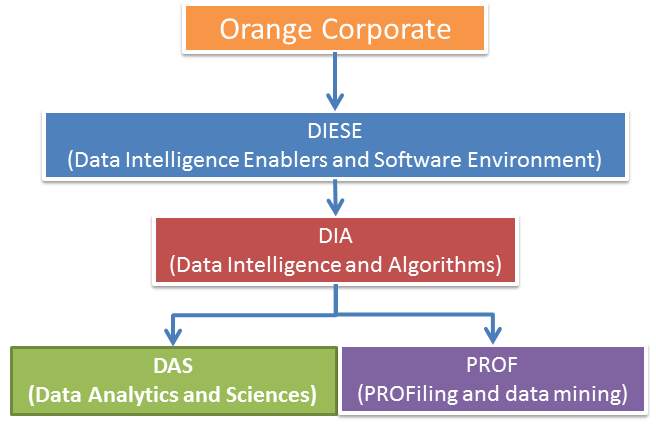
\includegraphics[scale=0.8]{schema_entites.png}\newline
	\end{center}
	J'effectue mon alternance dans la direction DIESE (Data Intelligence Enablers and Software Environment), dans les locaux de Châtillon baptisés "Orange Gardens". DIESE est une direction d'Orange Coporate qui est l'entité qui chapeaute tout le groupe Orange, notamment Orange France et les autres filiales d'Orange dans le monde ou encore Orange Business Service.
	L’objectif de DIESE est de fournir l’ensemble des ressources techniques, des services, des
	expertises et de l’accompagnement permettant à ces différentes entités de :
	\begin{enumerate}
		\item Traiter massivement l’ensemble des données disponibles,
		\item Mesurer en prédictif et en temps réel l’expérience client,
		\item Déployer en continu et en production tous les développements,
		\item Fournir des environnements de travail simples efficaces et favorisant l’agilité,
		\item Garantir une sécurité renforcée et de bout en bout des données.
	\end{enumerate}
	
	Au sein de DIESE j'ai rejoint le département DIA (Data Intelligence and Algorithms) qui contient cinq équipes dont deux sont notables pour la suite de ce mémoire :
	\begin{itemize}
		\item Mon équipe : DAS (Data Analytics and Sciences), dirigée par mon maître d'apprentissage Bruno Kauffmann. C'est une équipe de Data Scientists et Data Engineers qui ont un rôle d’expertise sur les projets de Data Science de toutes les entités du groupe.
		\item PROF (PROFiling and data mining) : C'est une équipe composée de chercheurs et d'ingénieurs de recherche dans le domaine du machine learning.
	\end{itemize}
	J'évolue donc dans un contexte très riche, entouré d'experts enthousiastes.
	\section*{Mission}
	Au sein de DAS mon rôle est d'assister les membres de l'équipe dans leurs divers projets. J'ai pendant cette première année pu participer à deux projets qui ont abouti avec succès :
	\begin{itemize}
		\item Un outil de pseudonymisation de données structurées
		\item Une library Python autour d'un outil de machine learning interne
	\end{itemize}
	J'ai participé à toutes les étapes de production d'un produit : de la caractérisation du besoin à la mise en production.
	
	L'objectif dans mes deux projets a été d'améliorer l'accessibilité à des technologies afin de les rendre utilisables par le plus grand nombre.
	Dans le premier projet, il a été question de mettre à la portée de presque n'importe qui la puissance du framework \textit{Apache Hadoop MapReduce} pour pseudonymiser des données. Le deuxième projet a quant à lui permis de rendre plus souple d'utilisation et plus attractif pour un certain public un logiciel de Machine Learning nommé \textit{Khiops} et développé par l'équipe PROF présentée précédemment.
	
	Durant cette première année j'ai découvert des aspects du métier de Data Engineer. Des missions avec une composante Data Science me seront sans doute confiées lorsque mon bagage de statistiques et de machine learning me le permettra au cours de l'année prochaine.
	
	\addcontentsline{toc}{section}{Mission}
	
	\newpage
	\chapter{Outil de pseudonymisation de données structurées}
	Entrons dans le vif du sujet avec une première partie détaillant le premier projet auquel j'ai participé. J'ai travaillé sur ce projet de septembre à février sous les conseils et en collaboration avec mon collègue Data Engineer Nebojsa Topolscak, projet suivi de près comme à son habitude par mon maître d'apprentissage Bruno Kauffmann.
	\section{Contexte et besoin}
	Rappelons rapidement les définitions des termes \textit{anonymisation} et \textit{pseudonymisation} d'après un article du site du CNRS \cite{cnrs}:
	
	\textit{L'anonymisation} des données détruit toute possibilité de pouvoir identifier à quel individu appartiennent les données personnelles. Ce processus consiste à modifier le contenu ou la structure des données en question afin de rendre la ré-identification des personnes quasi impossible, même après traitement.
	
	\textit{La pseudonymisation} est le traitement de données à caractère personnel de telle façon que celles-ci ne puissent plus être attribuées à une personne concernée précise sans avoir recours à des informations supplémentaires, pour autant que ces informations supplémentaires soient conservées séparément et soumises à des mesures techniques et organisationnelles afin de garantir que les données à caractère personnel ne sont pas attribuées à une personne physique identifiée ou identifiable.
	
	DIESE a été souvent sollicité pour de l'assistance à la pseudonymisation mais dans le contexte de nouvelle réglementation que constitue la mise en application le 25 Mai dernier du Règlement Général sur la Protection des Données, les demandes devenaient de plus en plus fréquentes. Dans la majorité des cas ces demandes portaient sur la pseudonymisation de données structurées\footnote{par opposition aux données brutes de type logs} de type CSV potentiellement massives. 
	
	Les clients potentiels sont des départements de DIESE ou des entités de filiales d'Orange qui ne disposent pas d'outil pour réaliser une pseudonymisation ou qui n'ont pas la capacité technique pour traiter de gros volumes.
	Nous avons commencé par répondre aux requêtes au cas par cas de façon personnalisée mais cette démarche n'était pas satisfaisante puisque trop chronophage dans le cas d’une forte demande. L'idée de Bruno a alors été de donner un outil aux clients pour les rendre autonomes. Le cahier des charges que doit remplir l'outil est le suivant:
	\begin{itemize}
		\item Être distribué pour passer à l'échelle
		\item Traiter tout type de fichier CSV
		\item Être facilement déployable sur les plateformes des clients
		\item Être suffisamment simple pour être utilisé par des employés peu techniques
	\end{itemize}
	
	\section{État de l'art}
	Nous allons faire ici un bref tour d'horizon des technologies disponibles pour nous rendre compte que notre cahier des charges nécessitait le développement d'un nouvel outil.
	
	\namedparagraph{Les solutions propriétaires}
	De nombreuses solutions propriétaires existent mais elles présentent souvent les mêmes désavantages. De plus, le fait qu'elles soient propriétaires est déjà problématique en soi. Nous allons en voir deux exemples assez représentatifs : 
	
	TeskaLabs a mis au point une solution nommée TurboCat.io() \cite{turbocat} qui  présente les avantages d'être très modulable et compatible avec une très grande variété d'environnements. Il n'est cependant pas distribué et ne peut donc pas passer à l'échelle du \textit{Big Data}. 
	
	La deuxième solution étudiée est Talend \cite{talend} qui est une solution puissante et tout en un qui gère le stockage, la pseudonymisation  et le traitement des données mais qui ne permet pas non plus un traitement distribué. De plus cette solution est assez lourde à mettre en place, ce qui est rédhibitoire pour un déploiement dans les filiales.
	
	
	\namedparagraph{Les solutions open source}
	Les solutions open source les plus pertinentes sont l'utilisation de projets de la fondation \textit{Apache} tels que \textit{Hive} ou \textit{Pig} qui sont des surcouches d'\textit{Hadoop} assez haut niveau. 
	
	Cependant ces technologies ne sont pas assez abstraites pour qu'un collaborateur peu technique les appréhende facilement. En effet, au-delà de la syntaxe non triviale, l'utilisation de ces technologies nécessite la définition de\textit{ User Defined Functions} (UDF) pour réaliser toutes les actions dont nous avons envie de disposer dans un outil de pseudonymisation, comme le \textit{hashing} qui n'est par exemple pas nativement supporté dans \textit{Pig}.
	
	Avec la même complexité d'utilisation nous pourrions envisager l'écriture de scripts \textit{Python} utilisant \textit{PySpark}.
	
	
	
	\section{Résolution de la problématique}
	
	Nous allons maintenant passer en revue les différentes étapes qui nous ont menés jusqu'à l'élaboration de la solution opérationnelle baptisée \textit{Pseudonymizer}.
	\subsection{Les premiers jobs customisés}
	Ma première tâche au sein de l'équipe a été de participer à l'apport d'une réponse au cas par cas aux besoins de pseudonymisations. La solution était d'écrire un job Hadoop MapReduce en Java 7 personnalisé pour chaque type de traitement. La méthode \textit{map} avait cette allure :
	\begin{lstlisting}
	public void map(LongWritable key, Text value, Context context) throws IOException, InterruptedException {
	// skip header (first line)
	if (key.get() == 0) {return;}
	//split line on separator FIELD_SEPARATOR
	String[] splittedLine = value.toString().split(FIELD_SEPARATOR);
	//Line process :
	StringBuffer modifiedLine=new StringBuffer();
	//Here we take the first 5 characters of the first field in clear and we hash the other part with SHA256
	modifiedLine.append(splittedLine[0].substring(0,5) + 
	HasherSha256.getHashAsBase64(seed,splittedLine[0].substring(5, splittedLine[0].length())));
	//We add a seperator
	modifiedLine.append(FIELD_SEPARATOR);
	//And so on for every field to process :
	[...]
	//the map returns modifiedLine by writing it to MapReduce context
	context.write(new Text(modifiedLine), NullWritable.get());
	}
	\end{lstlisting}
	Cette méthode devait être réécrite pour toute nouvelle demande en dialoguant avec le client afin de se mettre d'accord sur les actions à effectuer. Ensuite une fois notre job écrit et empaqueté dans un .jar, nous l'uploadions et l'exécutions sur le cluster de stockage et de calcul pour le Big Data géré par notre direction DIESE et nommé \textit{DIOD}. Le client pouvait ensuite accéder à ses données pseudonymisées sur la plateforme.
	
	Ce processus avait le gros désavantage de solliciter notre équipe pour un service à faible valeur ajoutée, potentiellement chronophage et pouvant être source d'erreurs d'incompréhension. Ces différents points ont donc justifié l'élaboration de l'outil qui fait l'objet de la section suivante.
	
	\subsection{Du premier prototype d'outil à la version industrielle} 
	\subsubsection{Le fichier de configuration}
	Bruno a lancé l'idée de l'utilisation d'un \textit{fichier de configuration}. L'utilisateur doit y renseigner les actions qu'il désire exécuter sur ses données et l'outil doit faire le reste du travail automatiquement.
	
	Il y a eu de nombreuses discussions auxquelles j'ai participé pour décider de la syntaxe à adopter pour ce fichier. Il fallait trouver une syntaxe simple et intuitive même pour un non développeur. Différentes tentatives ont été faites pour équilibrer la balance entre intuitivité et possibilités. Nous avons finalement décidé de nous inspirer de la syntaxe des fichiers de configuration du framework de traitement de logs \textit{Apache Flume}. 
	
	Voici un example de script basique pour notre outil:\newline
	\begin{lstlisting}[style=config]
	in.path = "WORK/Data/movies"  # définition du chemin vers le dossier d'input
	in.header = 1                   # indique la présence d'une ligne de header
	out.path = "WORK/Pseudo/movies_pseudonymized"  # chemin d'output
	out.separator = "\t"            # définition du séparateur en output
	log.path = "WORK/Pseudo/movies_job_logs"  # chemin pour les logs du traitement
	
	mon_sel_de_hachage = "toto"    # définition d'une variable contenant "toto"
	
	#  la 1ère  colonne de l'output est une copie de la 7ème  colonne d'input :
	out1 = in7  
	
	# la 2ème  colonne de l'output est le hash de la 3ème  colonne d'input :
	out2 = in3.hash(mon_sel_de_hachage)  
	\end{lstlisting}
	On voit donc qu'il y a globalement trois types de lignes : 
	\begin{itemize}
		\item Les lignes qui permettent de spécifier un paramètre du job: les chemins et les séparateurs dans cet exemple
		\item Les lignes qui permettent d'assigner une chaine de caractères à une variable : \newline \verb mon_sel_de_hachage="toto" .
		\item Les lignes qui permettent de définir le contenu d'une colonne du fichier résultat : \verb out1=in7 .
	\end{itemize}
	De nombreux opérateurs sont disponibles. Ils s'appliquent tous sur une chaine de caractères et renvoient également une chaine de caractères ce qui rends possible les cascades d'opérations. La seule exception est l'opérateur de concaténation \textbf{+} qui permet de joindre deux chaines. Avec ces opérateurs on peut facilement réaliser de nombreux traitements.
	Par exemple si la première colonne d'input contient une adresse email et que l'on souhaite hasher ce qu'il y a à droite du caractère \textbf{@} et garder le reste on va écrire :
	\begin{verbatim}
	in1.toChar("@").hash() + "@" + in1.fromChar("@")
	\end{verbatim}
	La figure suivante montre un autre exemple de fichier de configuration basique ainsi que le traitement des données qui lui est associé:
	\newline
	\begin{center}
		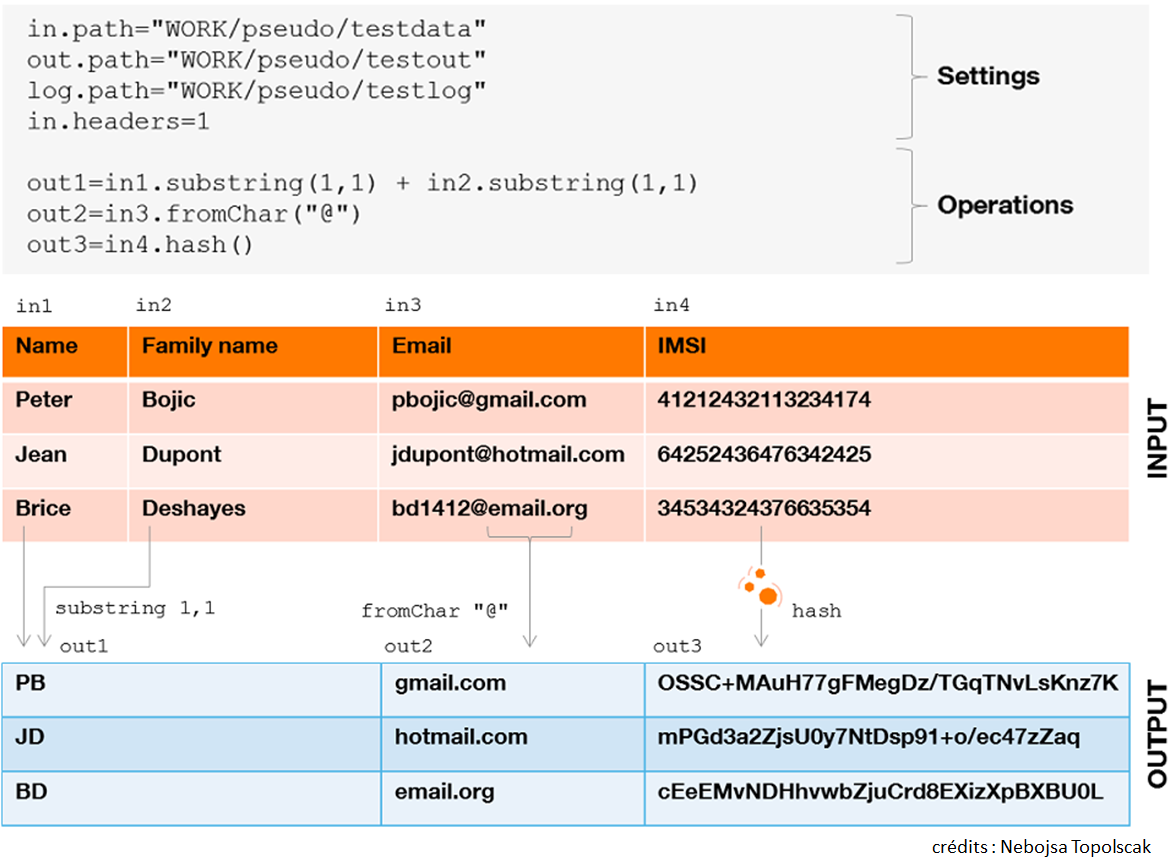
\includegraphics[scale=0.55]{configexample_.png}\newline
	\end{center}
	Une gestion des erreurs est également implémentée, prenons un exemple : Nous pouvons obtenir une sous-chaine de caractères entre la 5\textsuperscript{ème} et la 7\textsuperscript{ème}  position des champs de la colonne 1 à l'aide de l'opération \verb in1.substring(5,7) . Quel doit être le comportement de l'opération si le premier champ d'une des lignes ne contient par exemple que trois caractères ? Faut-il renvoyer une chaine vide ? Remplacer l'output par une autre chaine personnalisée ? Par un tag d'erreur ? Ou bien sauter cette ligne en la considérant comme invalide ? La réponse est que c'est à l'utilisateur de choisir et qu'il pourra le spécifier dans un paramètre optionnel à la fin de chaque opération. En reprenant l'exemple précédent, si l'on souhaite sauter la ligne dans le cas d'une erreur on écrira : \verb in1.substring(5,7,skipLine) .
	
	Cette syntaxe simple cache tout l'aspect technique à l'utilisateur mais reste néanmoins très modulable et puissante. Il y a une vingtaine d'options différentes spécifiables ainsi qu'une dizaine d'opérations. 
	
	\namedparagraph{Fonctionnalité avancée : Manipulation de tables de correspondances}
	Prenons ici un cas concret : Un service souhaite réaliser une étude pour déterminer des profils de fraudeurs. Le \textit{Pseudonymizer} sera un outil efficace pour hasher les champs sensibles en amont de l'étude afin que les Data Scientists ne manipulent pas de données en clair. Seulement il est primordial de pouvoir faire marche arrière une fois que leur modèle de détection sera opérationnel et que des identifiants hashés de fraudeurs seront remontés. 
	
	Une fonctionnalité existe pour combler ce besoin : la gestion de tables de correspondance. Ces tables établissent une correspondance entre les valeurs en clair et les hash. Étant donné un hash on pourra ainsi remonter vers l'identifiant si besoin. Ces tables sont des fichiers CSV qui devront être stockés dans un endroit hautement sécurisé et séparément des données pseudonymisées. Dans le fichier de configuration il suffit d'utiliser l'opération \verb .createHashMap(seed,map)  à la place de \verb .hash(seed)  pour activer la création d'une table de correspondance lors d'une opération de hash. Le retour en arrière se fait quant à lui à l'aide de l'opération \verb .lookup(map) .
	\subsubsection{Déploiement et utilisation}
	L'outil est facile à déployer pour un client puisqu'il ne comporte que deux éléments : une archive .jar contenant l'application ainsi qu'un petit script bash pour lancer l'outil proprement.
	Une fois son \textit{fichier de configuration} complété, l'utilisateur n'a ensuite qu'à lancer le script bash \textit{pseudo} avec le .jar et le \textit{fichier de configuration} en paramètres :\newline
	\begin{lstlisting}
	pseudo pseudonymizer-1.0.jar /path/configfile.txt
	\end{lstlisting}
	
	Dès que le traitement est terminé, l'utilisateur peut retrouver quelques logs sur le déroulement du traitement dans le dossier log qu'il a spécifié dans le fichier de configuration. En voici un exemple:
	
	\begin{verbatim}
	STAT:hdfs://PATH/name.csv	duration:976ms, linesTotal:100000, invalidLines:3,
	headersSkipped:0, fieldErrorsTotal:0, linesWithFieldErrors:0,
	invalidLinesBuffer:3/10(not saturated)
	
	hdfs://PATH/name.csv: INVALID_LINE 1: 130, unknown, 5
	hdfs://PATH/name.csv: INVALID_LINE 2: 5, unknown, 4
	hdfs://PATH/name.csv: INVALID_LINE 3: 268, unknown, 3
	\end{verbatim}
	Il peut y retrouver la durée du traitement ainsi que le compte de ses lignes ou des erreurs rencontrées. Un petit échantillon des lignes qui ont été considérées comme invalides est affiché pour donner une idée du problème à l'utilisateur.
	
	\subsubsection{Fonctionnement de l'outil}
	L'outil va ensuite se servir de ce fichier de configuration pour construire un job \textit{MapReduce} en suivant ces trois étapes :
	\begin{enumerate}
		\item Lexer et Parser le fichier de configuration pour créer du code source Java en mémoire capable de traiter une ligne d'input et de ressortir une ligne d'output. Des messages d'erreur précis sont affichés si des fautes syntaxiques ou des incohérences sont repérées et l'outil arrête immédiatement son exécution sans aller plus loin.
		\item Compiler \textit{à la volée} et toujours en mémoire cette chaine de caractères contenant le code source
		\item Créer une instance de la classe compilée obtenue et s'en servir pour traiter les lignes dans le \textit{Mapper} du job MapReduce
	\end{enumerate}
	\begin{center}
		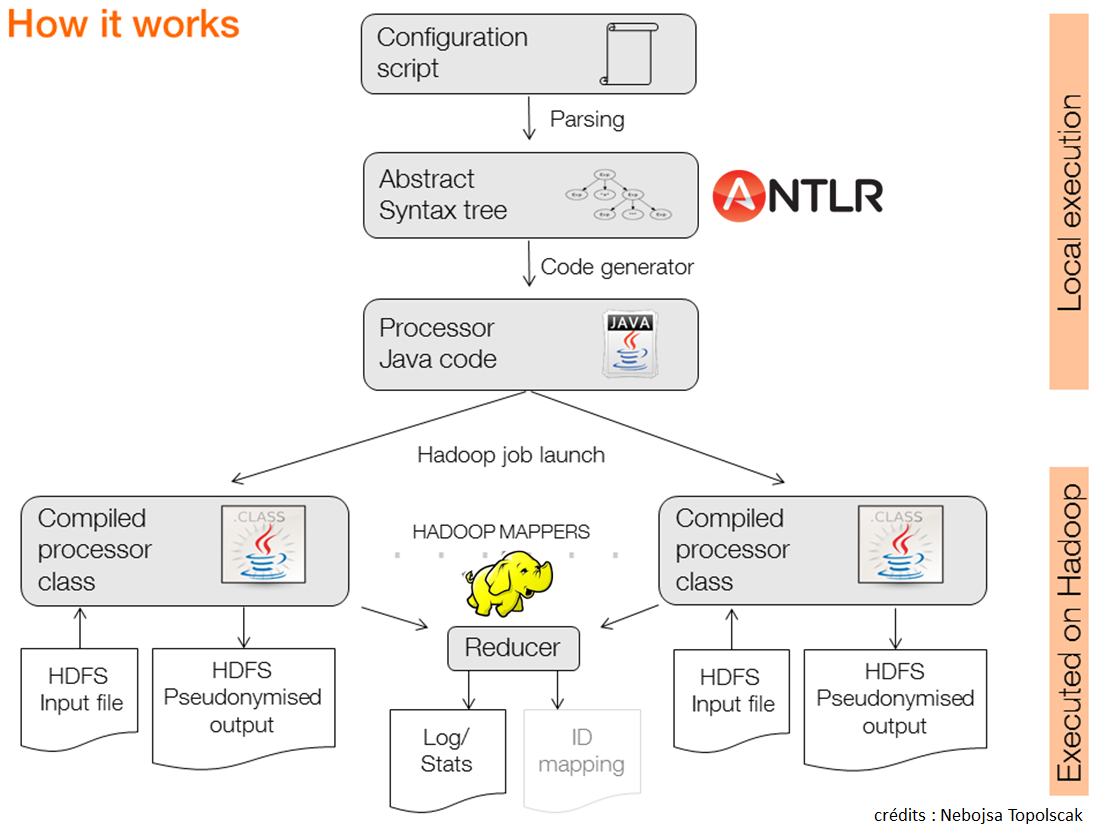
\includegraphics[scale=0.6]{pseudo_diag_.png}\newline
	\end{center}
	\subsubsection{Implémentation}
	\namedparagraph{Lexing et Parsing du fichier de configuration}
	Les premières versions de l'outil avaient des fonctionnalités assez limitées et ne permettaient par exemple pas de chainer des opérateurs ni d'effectuer des concaténations. J'ai donc dans un premier temps réalisé "à la main" le lexing et le parsing du fichier de configuration puisque la syntaxe était très basique. Cependant, au fur et à mesure que nous ajoutions des fonctionnalités à l'outil le code devenait impossible à maintenir. Nous sommes donc passé à l'utilisation d'un outil de parsing implémenté en Java nommé \textit{ANTLR}. Il permet de spécifier une grammaire et d'ensuite parcourir facilement l'arbre de syntaxe abstraite généré. Le code est devenu complètement industriel et l'ajout de nouvelles fonctionnalités est devenu trivial. La grammaire ANTLR utilisée est disponible en Annexe \ref{sec:grammaire}.
	\namedparagraph{I/O de fichiers CSV}
	La robustesse des IO est garantie par l'utilisation du package CSV d'Apache. L'outil gère grâce à lui la plupart des format csv, notamment le format d'export de csv d'\textit{Excel}. 
	\namedparagraph{Choix du langage et du framework de traitement distribué}
	Le langage Java a été choisi pour profiter de l'expertise de mon collègue Nebojsa. Le choix du framework \textit{Apache Hadoop MapReduce} plutôt qu'\textit{Apache Spark} a été quant à lui motivé par la plus grande maîtrise bas niveau qu'offre \textit{MapReduce} et par le fait que notre outil n'aurait pas bénéficié des optimisations qu'offre \textit{Spark} puisqu'il ne fait appel qu'à une seule phase de \textit{Map}.
	\namedparagraph{Choix de l'unité de division des données}
	Lorsque l'on réalise un traitement \textit{MapReduce}, l'unité de division des données est classiquement la ligne. Ce découpage implique naturellement que l'ordre des lignes de l'output ne correspond pas à celui de l'input et ceci était perçu comme un problème pour les clients. Il a alors été décidé de réalisé le \textit{split} avec pour unité le fichier. Ce choix a ralenti l'outil d'un facteur 1.5 à 2 mais était nécessaire.
	\newpage % fake
	\namedparagraph{Structuration}
	Nous avons développé le \textit{Pseudonymizer} en 6 packages qui contiennent en tout 25 classes, et un package de tests. 
	
	Le premier package nommé \textit{antlr} contient toutes les classes et interfaces générées par le framework \textit{ANTLR} et permettant le lexing et le parsing du fichier de configuration.
	
	Le package \textit{util} contient quant à lui les classes utilitaires permettant le hashage ou la gestion des tables de correspondance.
	
	Les quatre autres packages et leurs interconnexions sont décrits dans le tableau suivant au travers des classes principales qu'ils contiennent :\newline
	
	\begin{tabular}{|l|c|c|}
		\hline
		Classe & package & action \\
		\hline
		PseudoConfigVisitor & codegen & génère le code source Java du \textit{LineProcessor}\\
		&& à partir de l'arbre de syntaxe abstraite\\
		&&du fichier de configuration\\
		\hline
		PseudoConfigFactory&config&Factory permettant de créer une instance de \\
		&&\textit{PseudoConfig} à l'aide du \textit{PseudoConfigVisitor}\\
		\hline
		PseudoConfig&config&permet de stocker toutes les informations tirées du fichier\\
		&&de configuration durant son parsing. Contient le code  \\
		&&source \textit{Java} du \textit{LineProcessor}.\\
		\hline
		StreamProcessor & processor & permet de traiter, à l'aide du \textit{LineProcessor}, \\
		&&les lignes d'un stream de caractères issu des fichiers\\
		&& d'input et d'écrire dans un stream d'output vers le \textit{HDFS}\\
		\hline
		LineProcessor & processor & classe compilée à la volée par le  \textit{LineProcessorCompiler}\\
		&& à partir du code source généré par le \textit{PseudoConfigVisitor} \\
		\hline
		FullFileRecordReader & mr & étend la classe \textit{RecordReader} du framework\\
		&&MapReduce pour permettre de splitter les données\\
		&& avec le fichier pour unité plutôt que la ligne\\
		\hline
		PseudoMapper & mr &envoie les logs ainsi que les paires valeur-hash au \\
		&&\textit{PseudoReducer}. Mets en action le \textit{StreamProcessor}.\\
		
		\hline
		PseudoReduce & mr &Agrège les logs dans un fichier unique et rempli les\\
		&&tables de correspondance à partir des paires valeur-hash\\
		\hline
	\end{tabular}
	
	Voici un schéma des rôles des classes en amont du lancement du job MapReduce :
	\begin{center}
		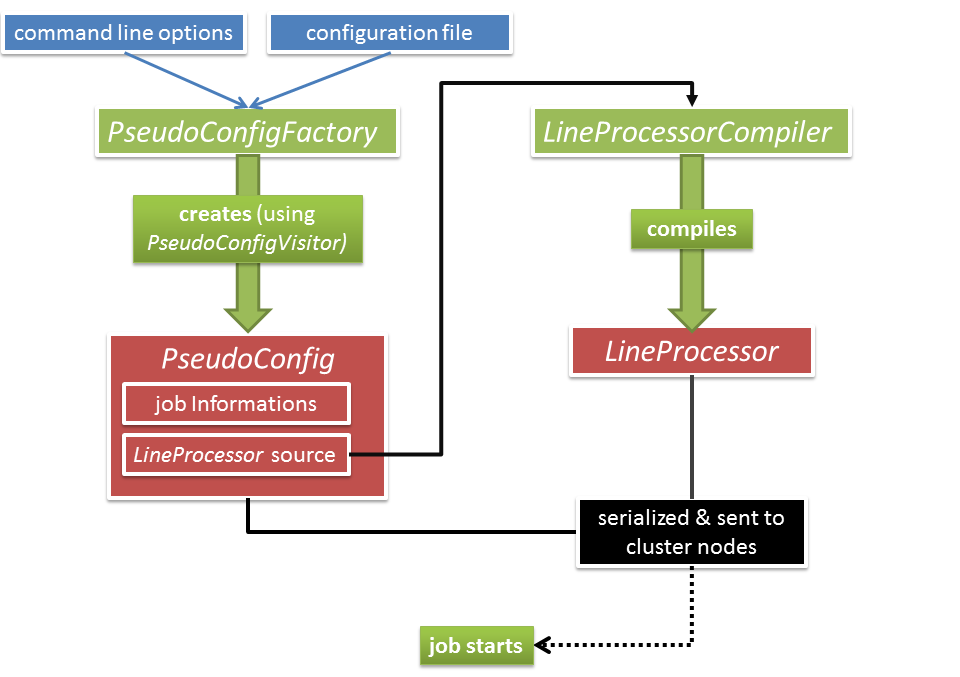
\includegraphics[scale=0.7]{schema.png}
	\end{center}
	Nous avons un \textit{design pattern} de \textit{'Factory'} pour la classe \textit{ConfigFileFactory}:
	\begin{lstlisting}
	public class PseudoConfigFactory {
	public static PseudoConfig createInstance(String configFileContent, CommandLine cline) throws PseudoConfigException{
	[...]
	return pseudoConfig;
	}
	}
	\end{lstlisting}
	\namedparagraph{Travail de documentation}
	L'élaboration d'une documentation utilisateur complète était une nécessité pour que l'outil soit utilisé. En effet même si il faut réaliser une présentation de l'outil au client pour motiver son adoption, il est primordial qu'il puisse être autonome, notamment pour la découverte des différentes fonctionnalités avancées. J'en ai rédigé une bonne partie et elle est accessible sur le wiki interne d'Orange. Vous pouvez la retrouver en Annexe \ref{sec:doc}.
	
	\section{Premiers résultats}
	Le \textit{Pseudonymizer} est souvent une alternative à une pseudonymisation non distribuée effectuée sur une machine. J'ai donc réalisé un benchmark pour comparer les performances de notre outil sur notre plateforme à celles d'un traitement écrit en \textit{C++} ou dans un script \textit{Python} et exécuté sur un processeur \textit{i7} récent. La pseudonymisation est réalisée sur un dossier de 416 fichiers de 100 Mo sur trois colonnes. L'action correspond aux lignes de configuration suivantes:
	\begin{lstlisting}[style=config]
	out1 = in2.toChar("(")
	out2 = in1 + in2.hash
	out3 = in2.substring(3, error)
	out4-6 = in1-3 
	\end{lstlisting}
	Le traitement contient des actions variées : recherche de caractère, concaténation, hashing, obtention de sous-chaine et recopie de 3 champs. Voici le résultat obtenu :
	\begin{center}
		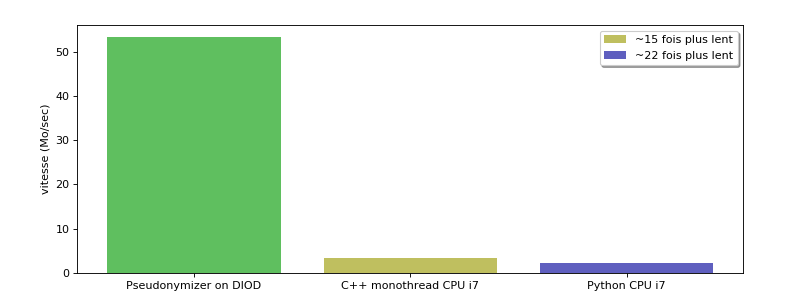
\includegraphics[scale=0.6]{bench.png}
	\end{center}
\underline{Note:} Les performances sur notre \textit{cluster} dépendent grandement de son état d'utilisation. Ainsi on peut décupler la vitesse du traitement en lançant l'outil sur une plage horaire peu exploitée. Ce benchmark n'est donné qu'à titre indicatif.
	
	L'outil commence à être utilisé en France par un département d'Orange Corporate ainsi que par un département d'Orange Côte d'Ivoire. J'ai demandé un retour au premier utilisateur de l'outil qui réalisait auparavant ses taches de pseudonymisation à l'aide d'un prétraitement \textit{Hive} : Il trouve que la syntaxe est assez complète pour son utilisation et que l’intérêt majeur de l'outil est qu'il permet dans son cas de découpler le chargement et le traitement des données sur la plateforme. \newline
	Il m'est arrivé dans ce contexte d'endosser le rôle de support pour conseiller notre client sur des aspects techniques liés à l'outil et sur la migration de leur ancienne solution vers notre outil.
	\section{Évolutions futures}
	\subsection{Chiffrement}
	Le principal désavantage de notre méthode de pseudonymisation réversible à base de tables de correspondances entre valeur en clair et valeurs hashées est le coup de stockage de ces tables. Permettre de chiffrer un champ pourrait donc s’avérer très pratique sur les jeux de données particulièrement massifs. 
	
	Il faudra forcément utiliser un mécanisme de chiffrement déterministe pour ne pas rendre impossible les agrégations selon le champ chiffré et perdre une grande partie de l'information contenue dans le jeux de données. Un chiffrement asymétrique pourrait également être très intéressant d'un point de vu sécurité puisque la clé publique manipulée par celui qui pseudonymise les données n'a pas une grande valeur tandis que la clé privée n'est utilisée qu'en cas de retours en arrière, potentiellement peu fréquents, et peut être stockée dans un endroit plus sûr. 
	
	Il faudra prévoir l'utilisation d'un sel comme dans le cas du hashage pour prévenir les attaques par \textit{dictionnaire} : une attaque par dictionnaire est une forme de brute force où l'attaquant connaissant l'algorithme utilisé va créer une table de correspondance avec des millions d'entrées, par exemple des millions de numéros de téléphone, afin de pouvoir les ré-identifier dans les données pseudonymisées. 
	
	\subsection{Traitement de données non et peu structurées}
	Une autre future amélioration concerne le traitement des logs. Les logs sont des données qui ne sont le plus souvent pas pré-structurées sous forme de colonnes. Ils nécessitent donc des mécanismes supplémentaires pour pseudonymiser les informations sensibles et identifiantes qu'ils contiendraient. 
	
	La plus basique des fonctionnalités pour réussir le traitement est l'utilisation d'expressions régulières. Grâce à elles nous serions capables de reconnaitre de nombreux patterns simples comme les numéros de téléphones ou les identifiants \textit{IMEI} des téléphones portables.
	
	Cependant il n'est par exemple pas possible avec une expression régulière de repérer des adresses de domicile dans un texte ne suivant aucun pattern précis. Nous avons pour cela planifié d'utiliser un modèle de \textit{champs aléatoires conditionnels} (CRF) pré-entrainé par les membres de NST, une autre équipe d'Orange Corporate. Ce modèle peut reconnaitre des adresses, des emails, des noms de familles et des prénoms. Nous pourrions également réaliser un autre entrainement afin de détecter des numéros de cartes bancaires ou encore permettre à l'utilisateur de fournir à l'outil un modèle de son choix.
	
	Une fois ces ajouts réalisés l'outil sera à même de couvrir une très grande partie des besoins du groupe, notamment la pseudonymisation de \textit{verbatim} issus de conversations avec les divers chatbots ou avec l'assistant d'Orange nommé \textit{Djingo}.
	
	\subsection{Version streaming}
	Une version streaming de l'outil est également planifiée pour permettre de connecter l'outil directement à l'ingestion des données sur la plateforme, par exemple par le biais d'un serveur \textit{Apache Kafka}, et d’éviter l'accumulation et le traitement de grosses quantités de données en une seule fois. Il s'agira de traitements en \textit{micro-batch} réalisés à l'aide d'\textit{Apache Spark}. Les changements pour adapter l'outil ne sont pas si lourds puisqu'il faudra remplacer la partie \textit{Hadoop MapReduce} par du \textit{Spark Streaming} mais que toutes les couches plus hautes comme le parsing du fichier de configuration et sa compilation en \textit{Java} restent inchangées.
	\newpage
	\chapter{Library Python autour d'un outil de machine learning}
	Abordons à présent le deuxième et dernier projet auquel j'ai pris part cette année, sous les conseils et en collaboration avec mon collègue chercheur en Data Science Alexis Bondu depuis le mois de Mars.
	\section{Contexte et besoin}
	\subsection{Qu'est-ce que Khiops ?}
	\textit{Khiops} est un outil de machine learning développé par l'équipe PROF depuis plus d'une décennie. Voici quelques caractéristiques :
	\begin{itemize}
		\item Il permet la classification, la regression et le clustering
		\item Il passe bien à l'échelle
		\item C'est un algorithme sans hyper-paramètres qui gère naturellement la balance entre biais et variance afin de ne pas tomber dans un sous-apprentissage ou sur-apprentissage
		\item Il permet d'apprendre sur des jeux de données composées de plusieurs tables
	\end{itemize}
	
	\namedparagraph{Note concernant le mode multitable de Khiops}
	Khiops va extraire des tables secondaires des agrégations les plus pertinentes possibles pour l'apprentissage. \newline
	Prenons un exemple : Imaginons que nous avons une table principale contenant des informations (âge, adresse, offre souscrite...) sur les clients possédant une carte SIM Orange et une table secondaire référençant les appels des clients. On souhaite savoir si les clients vont quitter Orange dans l'année qui suit ou bien rester à partir de ces données, afin de leur faire parvenir des offres ciblées attractives. Dans ce contexte \textit{Khiops} va par exemple détecter que le nombre d'appel de plus de 11 minutes effectués par un client durant le trimestres passé est une valeur très informative et l'utiliser lors de l'apprentissage.
	
	\subsection{Les limites ergonomiques de l'outil}
	Le mode d'utilisation classique de \textit{Khiops} se fait par le biais d'une interface graphique basées sur du Java Swing générée automatiquement :
	\begin{center}
		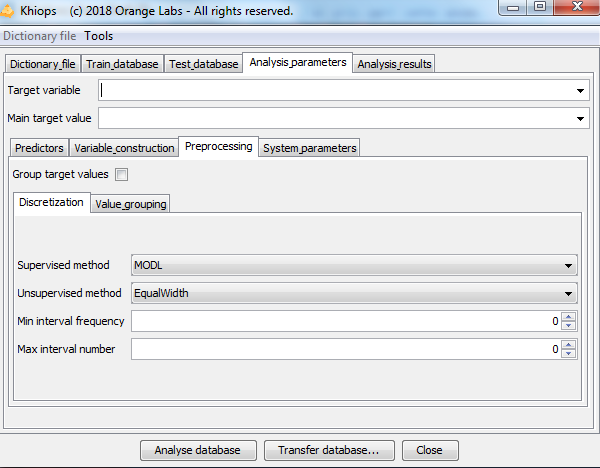
\includegraphics[scale=0.8]{screen_ihm_khiops.png}\newline
	\end{center}
	Les résultats sont quant à eux visualisables à l'aide d'un autre outil dédié.
	Les utilisateurs avertis de \textit{Khiops} ont la possibilité d'utiliser un langage de script propre à l'outil pour gagner du temps.
	
	Ces modes d'utilisation sont difficiles à prendre en main pour un néophyte habitué à manipuler les algorithmes de machine learning et leurs prédictions dans son langage de programmation.
	
	Ces limites ergonomiques gâchent et cachent la puissance de \textit{Khiops} aux yeux des potentiels nouveaux utilisateurs qui ne veulent pas dépenser du temps dans la prise en main d'un nouvel outil. Il semblait essentiel de pouvoir rendre plus attractif \textit{Khiops} en offrant un autre mode d'utilisation plus familier.
	\section{Solution apportée : PyKhiops}
	Alexis a alors réalisé dans ce contexte une première version de wrapper qui permet d'utiliser Khiops dans le langage \textit{Python} avec une syntaxe adoptant les conventions du framework très répandu \textit{scikit-learn}.
	Marc Boullé le créteur de \textit{Khiops} a par la suite fait mué ce projet de wrapper en une librairie complète permettant d'appeler toutes les fonctionnalités de \textit{Khiops} depuis un script \textit{Python}.
	
	Dans ce projet mon travail a été, sous la direction d'Alexis, de robustifier et d’industrialiser le module se chargeant de la partie wrapper \textit{scikit-learn}. J'ai ainsi :
	\begin{enumerate}
		\item Recodé l'ensemble du module pour qu'il adopte toutes les conventions \textit{pythoniques}.
		\item Refactorisé le code en fonctions élémentaires pour améliorer sa maintenabilité.
		\item Ajouté de nombreuses sécurités de typage et diverses vérifications de cohérence d'utilisation. Ce n'est pas \textit{pythonique} mais c'est essentiel pour que l'utilisateur ait des erreurs claires et qu'il n'ait pas une mauvaise image de \textit{Khiops} à cause du wrapper.
		\item Rédigé un set conséquent de tests unitaires
		\item Réalisé une documentation complète adoptant les conventions de \textit{scikit-learn}. Toute la documentation est factorisée dans la version de développement du module, c'est à dire que chaque paramètre de fonction n'est décrit qu'une seule fois pour une maintenabilité facilité. L'exécution de cette version de développement va générer une version \textit{release} du module avec une documentation lisible classique.
	\end{enumerate}
	
	Actuellement le module est finalisé et il sera rendu disponible nativement au sein de la librairie \textit{Python} complète dans la prochaine version de \textit{Khiops}.
	
	Voici un schéma qui représente le fonctionnement de la classe de classification \textit{PyKhiopsClassifier} :
	\begin{center}
		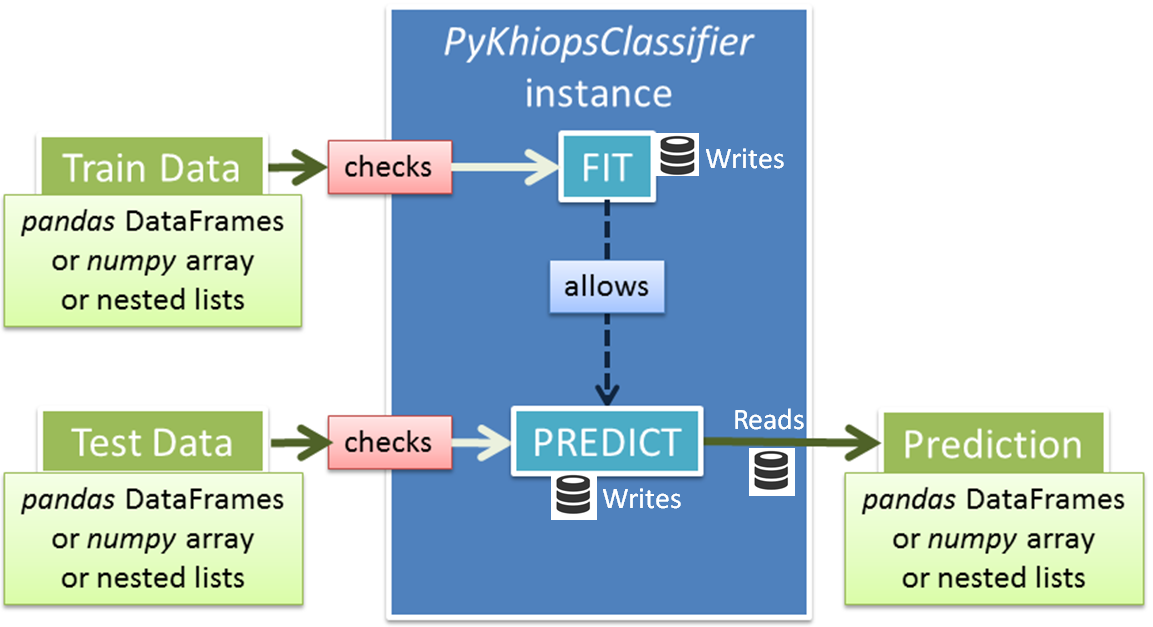
\includegraphics[scale=0.55]{pykhiops_.png}
	\end{center}
	Dans son utilisation basique de classification, le rôle du wrapper est :
	\begin{enumerate}
		\item de recevoir les données d'entrainement
		\item de réaliser des vérifications de typage et de dimension qui peuvent s'avérer complexes, notamment lorsque le mode \textit{multitable} est utilisé.
		\item d'écrire les données sur disque
		\item d'appeler \textit{Khiops} sur ces données pour obtenir un modèle entrainé
		\item de pouvoir ensuite recevoir des données de test
		\item de réaliser les mêmes vérifications que précédemment mais en vérifiant en plus la cohérence avec les données d'entrainement
		\item d'écrire les données sur disque
		\item d'appeler \textit{Khiops} sur ces données pour obtenir des prédictions à l'aide du modèle précédemment appris
		\item de récupérer ces prédictions depuis le disque et de les rendre à l'utilisateur sous la forme d'un objet \textit{Python} en cohérence de type avec les objets qu'il a fourni jusqu'à présent
	\end{enumerate}
	
	Voici un exemple de script utilisant le module :
	\begin{lstlisting}[style=py]
	from PyKhiops import PyKhiopsClassifier, acc
	import pandas as pd
	
	X_train, y_train, X_test, y_test = [charge données avec pandas]
	
	pk = PyKhiopsClassifier()
	pk.fit(X=X_train, y=y_train)
	y_pred = pk.predict(X=X_test)
	print(acc(y_pred, y_test))  # on regarde l'accuracy de la prédiction
	\end{lstlisting}
	
	La syntaxe pour du \textit{multitable} a été pensée pour être très simple et tirer parti de l'indexation des DataFrames du module \textit{pandas} : 
	
	\begin{lstlisting}[style=py]
	#On souhaite ici prédire l'age de clients à partir d'une table principale et
	#d'une table secondaire d'appels passés et d'une table de factures hors forfait :
	from PyKhiops import PyKhiopsClassifier, acc
	import pandas as pd
	
	clients_train, appels_train, hors_forfaits_train, age_train,
	clients_test, appels_test, hors_forfaits_test, age_test = [charge données avec pandas]
	
	pk = PyKhiopsClassifier()
	pk.fit(X=clients_train, X_list=[appels_train, hors_forfaits_train] y=age_train)
	age_pred = pk.predict(X=clients_test, X_list=[appels_test, hors_forfaits_test])
	print(acc(age_pred, age_test))
	\end{lstlisting}
	
	Ce module rend donc très familière l'utilisation de \textit{Khiops} pour n'importe quel Data Scientist.
	Le module permet également d'utiliser la classe \textit{PyKhiopsRecoder} qui est un wrapping de la fonctionnalité de \textit{Khiops} de recodage de jeux de données.
	
	\section{Évolutions futures}
	La librairie est déjà utilisée par les différents stagiaires de l'équipe et quelques améliorations sont prévues pour mon module comme par exemple l'ajout d'une classe PyKhiopsRegressor pour compléter les possibilités d'apprentissage supervisé du wrapper.
	
	Il se pourrait également la fonctionnalité de coclustering de \textit{Khiops} soit prochainement wrappée pour \textit{Spark} en \textit{Scala}. Il sera alors pertinent d'ajouter à la librairie \textit{PyKhiops} un module \textit{PySparkKhiops}...
	
	\newpage
	\chapter{Enseignements tirés et progression personnelle sur cette 1ère année}
	Durant cette année, je me suis vraiment senti progresser durant chacune de mes sessions en entreprise. J'ai gagné en expérience technique autant qu'en expérience du monde de l'entreprise.
	\section{Vie d'entreprise}
	J'en sais désormais plus sur le fonctionnement d'un grand groupe tel qu'Orange et sur les bonnes pratiques à adopter pour être efficace dans un tel environnement. Il faut être à l'écoute de ses collaborateurs et ne pas se précipiter. Le temps dépensé à prendre du recul sur une tâche et à en discuter est très largement rattrapé par la suite. J'ai la chance de pouvoir être entouré de collègue experts et patients qui m'apportent leur conseils dès que nécessaire. 
	\section{Technique}
	Je vais ici essayer de récapituler brièvement les progressions techniques que j'ai effectuées lors de mes sessions d'entreprise de cette année. 
	\subsection{Java}
	Aux côtés de mon collègue Nebojsa j'ai énormément progressé en développement \textit{Java} et en génie logiciel.
	
	J'ai appris à écrire un code modulaire en structurant le code en classes ayant un rôle naturel et utilisant si nécessaire des \textit{design patterns} pertinents. Le code est ainsi facilement maintenable et lisible, ce qui est essentiel lorsque nous sommes plusieurs à collaborer sur le même projet. J'ai également appris qu'il faut éviter à tout prix de réinventer la roue. Il est très rentable de passer du temps à rechercher des solutions existantes pour ensuite les adapter.
	
	J'ai également intégré des détails d'optimisation tels que l'utilisation d'énumérations ou de \textit{StringBuffer} pour construire des chaines de caractères efficacement. J'ai gagné en compétence sur le framework\textit{ Apache Hadoop}, que ce soit au niveau \textit{HDFS} ou \textit{MapReduce}. L'utilisation dans un contexte industriel d'une grammaire de langage de script à l'aide d'\textit{ANTLR} a aussi été enrichissante.
	
	\subsection{Python}
	Grâce notamment à Eole et Alexis j'ai beaucoup progressé en développement \textit{Python} jusqu'à être capable de produire un code industriel. J'en suis presque arrivé à connaître par coeur les Python Enhancement Practices...
	
	J'ai appris à gérer la balance entre optimisations fines et lisibilité. Un code \textit{Python} se doit dans la plupart des cas d'être lisible et compréhensible en l'absence de commentaires, quitte à sacrifier quelques millisecondes lors de l'exécution. 
	
	J'ai également dû me familiariser avec énormément de détails des packages \textit{numpy} et \textit{pandas} ainsi qu'avec le module \textit{unittest}.
	
	\newpage
	\chapter*{Conclusion}
	Cette première année m'a conforté dans l'idée que l'alternance est vraiment un processus d'apprentissage qui me correspond. Je me suis tout autant enrichi au cours des sessions universitaires qu'au cours des sessions en entreprise. Pouvoir mettre en application dans un contexte professionnel ce que l'on apprend est vraiment valorisant et permet de se remettre en question en permanence.
	
	Mes deux projets de l'année m'ont énormément appris techniquement sur des aspects variés s'étalant sur tout le cycle de production d'un outil industriel.
	
	Je vais profiter de ma dernière année de Master en apprentissage pour parfaire mon bagage technique et gagner un maximum de compétences et d'expérience afin de prétendre à devenir un Data Engineer efficace !
	
	\addcontentsline{toc}{chapter}{Conclusion}
	\newpage
	\bibliographystyle{plain} % Le style est mis entre accolades.
	\bibliography{memoire_m1} % mon fichier de base de données s'appelle bibli.bib
	\newpage
	\chapter{Annexe}
	
	\section{Grammaire du fichier de configuration du Pseudonymizer}
	\label{sec:grammaire}
	Voici le fichier .g4 décrivant notre grammaire pour le framework \textit{ANTLR}.
	\noindent
	\begin{lstlisting}[style=py, gobble=1]
	grammar Pseudo;
	
	configFile: assignment+ EOF;
	
	assignment:      
	IN_FIELDS '=' INT                              #AssignInFields
	|IN_PATH '=' STRING                            #AssignInPath
	|IN_SEPARATOR '=' STRING                       #AssignInSeparator
	|IN_HEADERS '=' INT                            #AssignInHeaders
	|OUT_KEEPHEADERS '=' INT                       #AssignOutKeepHeaders
	|OUTXHEADER '=' STRING                         #AssignOutXHeader
	|IN_NAMES '=' varlist                          #AssignInNames
	|IN_ENCODING '=' STRING                        #AssignInEncoding
	|IN_CSVTYPE '=' csvType = (K_EXCEL|K_TSV|K_RFC)#AssignInCsvType
	|OUT_PATH '=' STRING                           #AssignOutPath
	|OUT_SEPARATOR '=' STRING                      #AssignOutSeparator
	|OUT_SEED '=' outSeed = (STRING|K_RANDOM)      #AssignOutSeed
	|OUT_ERROR '=' STRING                          #AssignOutError
	|OUT_ENCODING '=' STRING                       #AssignOutEncoding
	|OUT_CSVTYPE '=' csvType =(K_EXCEL|K_TSV|K_RFC)#AssignOutCsvType
	|LOG_PATH '=' STRING                           #AssignLogPath
	|MAP_COLLISION '=' collisionCheck=(K_ON|K_OFF) #AssignCollisionCheck
	|VAR '=' concat                                #AssignVar
	|OUTVAR '=' concat                             #AssignOutVar
	|mapVar=MAPVAR '.path' '=' STRING              #AssignMapPath
	|OUTRANGE '=' INRANGE                          #AssignRange
	; 
	
	concat: tok | (tok '+' concat); 
	
	tok:    tokvar(f_substring2|f_substring3
	|f_last|f_tochar|f_fromchar
	|f_hash0|f_hash1
	|f_createhashmap1|f_createhashmap2
	|f_lookuporcreatehashmap1|f_lookuporcreatehashmap2|f_lookup)*?;
	
	tokvar: 
	VAR       #TokvarVar 
	|INVAR    #TokvarInvar
	|STRING   #TokvarString
	;
	
	varlist: VAR (',' VAR)*;
	
	f_substring2:   			     
	'.substring(' arg1=INT (',' arg2=(K_ALL|K_ERROR|K_SKIP|STRING))?')';
	f_substring3: '.substring('arg1=INT','arg2=INT(','arg3=(K_ALL|K_INTERSECTION|K_ERROR|K_SKIP|STRING))?')';
	f_last:         			     
	'.last('arg1=INT(','arg2=(K_ALL|K_INTERSECTION|K_ERROR|K_SKIP|STRING))?')';
	f_tochar:      				     
	'.toChar(' arg1=STRING (',' arg2=(K_ALL|K_ERROR|K_SKIP|STRING))?')';
	f_fromchar:    				     
	'.fromChar(' arg1=STRING (',' arg2=(K_ALL|K_ERROR|K_SKIP|STRING))? ')';
	f_hash0:        			     
	'.hash'|'.hash(' ')';
	f_hash1:        			     
	'.hash(' arg1=STRING ')';
	f_createhashmap1:			     
	'.createHashMap(' arg1=MAPVAR ')';
	f_createhashmap2:			     
	'.createHashMap(' arg1=MAPVAR ',' arg2=STRING ')';
	f_lookuporcreatehashmap1:	 
	'.addToHashMap(' arg1=MAPVAR')';
	f_lookuporcreatehashmap2:	 
	'.addToHashMap(' arg1=MAPVAR ',' arg2=STRING')'; 
	f_lookup:					         
	'.lookup(' arg1=MAPVAR (',' arg2=(K_ERROR|K_SKIP|STRING))?')';
	
	K_ALL:            'all';
	K_INTERSECTION:   'intersection';
	K_ERROR:          'error';
	K_SKIP:           'skipLine';
	K_RANDOM:         'random';
	K_EXCEL:          [eE][xX][cC][eE][lL];
	K_TSV:            [tT][sS][vV];
	K_RFC:            [rR][fF][cC];
	K_ON:             [oO][nN];
	K_OFF:            [oO][fF][fF];
	
	IN_FIELDS:             'in.fields';
	IN_PATH:               'in.path';
	IN_SEPARATOR:          'in.separator';
	IN_HEADERS:            'in.headers';
	OUT_KEEPHEADERS:       'out.keepHeaders';
	IN_NAMES:              'in.names';
	IN_ENCODING:           'in.encoding';
	IN_CSVTYPE:            'in.csvType';
	OUT_PATH:              'out.path';
	OUT_SEPARATOR:         'out.separator';
	OUT_SEED:              'out.seed';
	OUT_ERROR:             'out.error';
	OUT_ENCODING:          'out.encoding';
	OUT_CSVTYPE:           'out.csvType';
	LOG_PATH:              'log.path';
	MAP_COLLISION:         'map.collisionCheck';
	OUTXHEADER:            'out'[0-9]+'.header';
	
	BOOL:       ('true'|'false');
	INRANGE:    'in' [0-9]+ '-' [0-9]+;
	OUTRANGE:   'out' [0-9]+ '-' [0-9]+;
	INVAR:      'in' [0-9]+ ;
	OUTVAR:     'out' [0-9]+;
	MAPVAR:     'map'[0-9]+;
	STRING:     '"' ('\\"'|~'"')* '"' ; // backslash-quote is an escaped quote
	INT:        [0-9]+ ;
	VAR:        ([a-z]|[A-Z])([a-z]|[A-Z]|[0-9]|'-'|'_')*; //1st char must be alpha
	EOL:        '\r'? '\n' -> channel(HIDDEN);
	WS:         (' ' | '\t')+ -> channel(HIDDEN);
	COMMENT:    '#'.*?( EOL|EOF) -> channel(HIDDEN);
	\end{lstlisting}
	
\end{document}
